\documentclass[a4paper,10pt,spanish,oneside]{article}

% Preámbulo - Parte A

\usepackage[utf8]{inputenc} % Soporte para los acentos
\usepackage[T1]{fontenc}

\usepackage[spanish]{babel} % Capítulos, seciones, etc. en español

\usepackage[margin=1.5cm]{geometry} % Diseño del documento

\usepackage{multicol} % Escribir doble columna

\usepackage{xcolor} % Usar colores
\usepackage{pstricks}

\usepackage{enumerate} % Cambiar etiquetas de numeración
\usepackage[shortlabels]{enumitem} % Manejo adicional de etiquetas de numeración

\usepackage{graphicx} % Manejo de gráficos y figuras

\usepackage{makeidx} % Índice alfabético

% Paquetes adicionales de símbolos matemáticos
\usepackage{amsmath,amssymb,amsfonts,latexsym,cancel} 

% \usepackage{pslatex} % Fuente Times
% \usepackage{mathpazo} % Fuente Palatino
% \usepackage{mathptmx} % Fuente Times
% \usepackage{bookman} % Fuente Bookman
\usepackage{newcent} % Fuente New Century Schoolbook
% \usepackage{helvet} % Fuente Helvetica
% \usepackage{palatino} % Fuente Palatino
% \usepackage{pxfonts} % Fuente 
% \usepackage{txfonts} % Fuente
% \usepackage{concrete} % Fuente
% \usepackage{cmbright} % Fuente
% \usepackage{fourier} % Fuente

\usepackage{booktabs} % Opciones adicionales para el entorno tabular
\usepackage{longtable} % Para tablas de más de una página

\usepackage{tikz} % Creación de gráficos

% \usepackage{titlesec} % Personalizar capítulos y secciones

% Preámbulo - Parte B

\pagestyle{headings}

%\pagestyle{myheadings} % Numeración de página en la parte superior

%\usepackage{titlesec}

%\titleformat{\section} % command
%			[display] % shape
%			{\usefont{T1}{phv}{b}{n}\LARGE} % format
%			{} % label
%			{1pt} % sep
%			{\thesection.\hspace{0.5em}} % before code
%			
%\titleformat{\subsubsection} % command
%			[display] % shape
%			{\usefont{T1}{phv}{b}{n}\Large} % format
%			{} % label
%			{1pt} % sep
%			{\thesubsection.\hspace{0.5em}} % before code
%			
%\titleformat{\subsubsection} % command
%			[display] % shape
%			{\usefont{T1}{phv}{b}{n}\large} % format, fuentes: lmss,pag,phv
%			{} % label
%			{1pt} % sep
%			{\thesubsubsection.\hspace{0.5em}} % before code		
%
%\titleformat{name=\section,numberless}
%			[display]
%			{\usefont{T1}{phv}{b}{n}\LARGE}
%			{}
%  			{1pt}
%  			{}
%			\titlespacing*{\section}{0pt}{1pt}{1pt}

%%---
%\usepackage{geometry} %Algo de las líneas del pie y encabezados
%\geometry{text={7in,9.5in},headheight=15pt}
%%\textwidth = 7 in
%%\textheight = 9.5 in
%%\oddsidemargin = -0.25 in
%%\evensidemargin = 0.0 in
%%\topmargin = -0.25 in
%%\headheight = 0.0 in
%%\headsep = 0.0 in
%\setlength{\parskip}{0.1in}
%\setlength{\parindent}{0.0in}
%%---
%\usepackage{fancyhdr} %Para usar encabezados y pies personalizados
%	\pagestyle{fancy}
%	\fancyhf{}
%	% E: par
%	% O: impar
%	\fancyhead[LE,RO]{Inteligencia Computacional} 
%	\fancyhead[RE,LO]{Preguntas del primer parcial}
%	\fancyfoot[RE,LO]{Darién Julián Ramírez, Gaspar Oberti, Marcos Pereira}
%	\fancyfoot[LE,RO]{\thepage}
%	\renewcommand{\footrulewidth}{1pt}
%%---

%\usefont{T1}{lmss}{b}{n}

\title{\Huge Inteligencia Computacional\\
Parcial 1}
\author{Marcos Pereira, Gaspar Oberti y Darién Julián Ramírez}
\date{\vspace{-5ex}}

\begin{document}

\maketitle %Crea la página de título

\tableofcontents

\newpage

\section{Unidad I - Introducción}

\begin{itemize}
\item Breve revisión histórica a la inteligencia computacional.
\item Áreas del conocimiento involucradas y su relación como parte de la inteligencia artificial.
\item El cerebro humano y las limitaciones del cálculo computacional.
\item El impacto y el amplio espectro de aplicaciones de la inteligencia computacional.
\item Introducción conceptual a las tres técnicas fundamentales de la inteligencia computacional.
\end{itemize}

\subsection{Introducción}

\begin{enumerate}
\item (6) ¿Qué diferencias hay entre inteligencia artificial e inteligencia computacional?

\item (3) Clasifique tipos y reglas de aprendizaje, ejemplificando en cada caso.

\item (3) Clasificación de las arquitecturas de redes neuronales. En cada caso indique cuáles algoritmos de entrenamiento son aplicables.

\item (3) Enumere problemas prácticos que el ser humano aún hoy resuelve mejor que una computadora.
\end{enumerate}

\newpage

\section{Unidad II - Redes Neuronales I}

\begin{itemize}
\item Bases estadísticas del reconocimiento de patrones: etapas, decisión bayesiana, funciones discriminantes.
\item Aprendizaje, espacio de soluciones, mínimos locales y globales, capacidad de generalización y técnicas de validación cruzada.
\item La inspiración biológica en redes neuronales: fisiología neuronal básica, redes de neuronas biológicas y escalas de organización estructural del cerebro.
\item Modelos de neurona: la sinapsis, funciones de activación. Perceptrón simple: hiperplanos para la separación de clases, entrenamiento y limitaciones.
\item Generalidades: características de las redes neuronales, clasificación de las arquitecturas neuronales, clasificación de los procesos de aprendizaje.
\end{itemize}

\subsection{Perceptrón simple}

\subsubsection{Video 001 - Fisiología básica de una neurona}

\begin{enumerate}
\item ¿A qué se denomina robustez y a qué capacidad de adaptación en los sistemas inteligentes (redes neuronales)?

\item ¿Qué es la capacidad de generalización en una red neuronal?

\item Enumere tres diferencias entre los métodos de cálculo del cerebro y los de una computadora.
\end{enumerate}

\subsubsection{Video 002 - Modelo simplificado de neurona}

\begin{enumerate}
\item (8) Describa qué es la despolarización de una neurona y como llega a producirse. Liste las principales simplificaciones (3) que se hacen en el modelo del perceptrón simple (en comparación con la neurona biológica).

\item ¿Qué es el árbol dendrítico de una neurona y cómo se modela en el preceptrón simple?

\item ¿Cómo se simplifica la dinámica temporal en un modelo de perceptrón simple?

\item Describa las diferentes funciones de activación que conoce.
\end{enumerate}

\subsubsection{Video 003 - Un perceptrón simple con dos entradas}

\begin{enumerate}
\item (8) Muestre con un ejemplo cuáles son las limitaciones de un perceptrón simple en tareas de clasificación (ecuaciones e interpretación gráfica).

\item (2) ¿Cuál es la importancia del sesgo en un perceptrón simple? Explique con un ejemplo.
\end{enumerate}

\subsubsection{Video 004 - Algoritmos de aprendizaje (PS)}

\begin{enumerate}
\item ¿Qué rol cumple el principio de mínima perturbación en el entrenamiento de un perceptrón simple?
\end{enumerate}

\subsubsection{Video 005 - Método de gradiente (PS)}

\begin{enumerate}
\item (5) Obtenga la ecuación de actualización de pesos para el perceptrón simple, considerando una función de activación lineal.

\item Muestre con un ejemplo numérico cómo el algoritmo de entrenamiento del perceptrón simple ajusta los pesos haciendo que el error se reduzca.
\end{enumerate}

\subsection{Introducción al reconocimiento estadístico de patrones}

\subsubsection{Video i04 - Clasificación estadística}

\begin{enumerate}
\item ¿A qué se denomina clasificador estadístico? Defina y represente gráficamente.
\end{enumerate}

\subsubsection{Videos i05 y i06 - Teoría de la decisión y Clasificador de Bayes}

\begin{enumerate}
\item (3) ¿Qué es un clasificador de Bayes? Defina y explique.

\item Explique cómo aplicar el clasificador de Bayes al problema de Iris.
\end{enumerate}

\subsection{Capacidad de generalización}

\subsubsection{Video a01 - Superficies de error}

\begin{enumerate}
\item (4) ¿Qué es la capacidad de generalización, qué importancia tiene y cómo puede medirse?

\item (2) ¿Qué son los mínimos locales y qué métodos conoce para evitarlos?

\item ¿Qué son, como se construyen y para qué se utilizan los conjuntos de entrenamiento, prueba y monitoreo?
\end{enumerate}

\subsubsection{Video a02 - Sobreentrenamiento 1}

\begin{enumerate}
\item (3) Desarrolle el concepto de sobre-entrenamiento en relación a la cantidad de parámetros libres y a la cantidad de épocas de entrenamiento ¿Cómo se puede evitar?

\item ¿Qué es el sobre-entrenamiento y qué relación tiene con los mínimos locales?
\end{enumerate}

\subsubsection{Video a04 - Estimación de la capacidad de generalización}

\begin{enumerate}
\item (6) ¿Cuál es la importancia práctica de los \textit{métodos de estimación del error} (validación cruzada y sus variantes)? ¿Qué hipótesis debe relajarse para poder realizar 10 particiones con relación 80/20?

\item (2) ¿Por qué se realizan múltiples particiones en la validación cruzada? ¿Cuál es el impacto de aumentar la cantidad de particiones en la estimación del error de clasificación?

\item (2) ¿Cuál es el problema que puede surgir a partir de la utilización de una única partición de entrenamiento y prueba?

\item ¿Cómo realizaría el entrenamiento y validación cruzada en el caso de que una de las clases tenga muchos más ejemplos que las otras?
\end{enumerate}

\subsubsection{Video a05 - Variantes de la validación cruzada}

\begin{enumerate}
\item (3) Describa dos métodos de validación cruzada. ¿Para que sirve y cómo se utiliza el conjunto de monitoreo?
\end{enumerate}

\newpage

\section{Unidad III - Redes Neuronales II}

\begin{itemize}
\item Perceptrón multicapa: formulación matemática del algoritmo de retropropagación, velocidad de aprendizaje y término de momento, inicialización y criterios de finalización, definición de la topología y los parámetros de entrenamiento.
\item Redes neuronales con funciones de base radial: arquitectura, fronteras de decisión, algoritmos de entrenamiento.
\item Mapas auto-organizativos: arquitecturas, algoritmo de entrenamiento, mapas topológicos, cuantización vectorial con aprendizaje, comparación con otros métodos de agrupamiento.
\item Redes neuronales dinámicas: redes de Hopfield, retropropagación a través del tiempo, redes neuronales con retardos en el tiempo.
\end{itemize}

\subsection{Perceptrón multicapa}

\subsubsection{Videos 006, 007 y 008 - Problema XOR con 3 neuronas, Nuestra primera red neuronal (un perceptrón multicapa con 3 neuronas) y ¿Y resolverá el XOR?}

\begin{enumerate}
\item (6) Encuentre la estructura neuronal mínima para resolver el problema XOR y deduzca un conjunto de pesos adecuado. Represente gráficamente las regiones de decisión.

\item (2) Describa las limitaciones de un perceptrón simple y la forma de sortearlas mediante la combinación de varios perceptrones.
\end{enumerate}

\subsubsection{Video 009 - Perceptrón multicapa (MLP), regiones de decisión, arquitectura}

\begin{enumerate}
\item (3) Represente gráficamente el tipo de regiones que puede separar un perceptrón multicapa en función de la cantidad de capas ocultas que posee, comenzando por el perceptrón simple (1, 2 y 3 capas). Explique a qué se deben las limitaciones de cada arquitectura.

\item (2) ¿Qué tipo de problemas no pueden ser resueltos por una arquitectura de dos capas?
\end{enumerate}

\subsubsection{Videos 010 y 011 - Propagación hacia atrás (caso general) y Aplicación del gradiente}

\begin{enumerate}
\item (6) Defina matemáticamente el gradiente de error local instantáneo, y obtenga su forma general para una función de activación sigmoidea simétrica y describa cuál es su importancia en el algoritmo de retropropagación.

\item (2) ¿Qué es el gradiente de error local instantáneo y que rol juega en el algoritmo de retropropagación?
\end{enumerate}

\subsubsection{Video 012 - Retropropagación en la capa III (Salida)}

\begin{enumerate}
\item (6) Obtenga la ecuación de actualización de pesos para el perceptrón simple, considerando una función de activación sigmoidea.

\item Demuestre la ecuación del algoritmo de retropropagación para la última capa de un perceptrón multicapa.
\end{enumerate}

\subsubsection{Video 013 - Propagación hacia atrás (Capas ocultas)}

\begin{enumerate}
\item (4) Obtenga la ecuación de actualización de pesos para la capa oculta de un perceptrón multicapa.
\end{enumerate}

\subsubsection{Video 014 - Resumen del algoritmo de retropropagación (BP)}

\begin{enumerate}
\item Escriba el algoritmo de entrenamiento de un perceptrón multicapa.

\item (3) Explique conceptual y gráficamente el proceso de retropropagación del error para perceptrones multicapa de $2, 3,..., N$ capas.
\end{enumerate}

\subsubsection{Constante de momento: $\Delta w_{ji}(n)={\red \alpha\Delta w_{ji}(n-1)}-\eta\frac{\partial\xi(n)}{\partial w_{ji}(n)}$}

\begin{enumerate}
\item (6) ¿Cómo se incluye el término de momento en el algoritmo de retropropagación? Explique su función en la navegación por la superficie de error.

\item Explique cuál es el problema con la existencia de mínimos locales para el entrenamiento de un perceptrón multicapa ¿De que aspectos depende este problema? Proponga al menos dos alternativas para reducir su efecto en el entrenamiento.
\end{enumerate}

\subsection{Redes con funciones de base radial}

\subsubsection{Video 015 - Redes neuronales con funciones de base radial}

\begin{enumerate}
\item (4) Compare las fronteras de decisión que pueden construirse a partir de un perceptrón multicapa con las de una red neuronal con funciones de base radial ejemplificando casos donde una es mejor que la otra y viceversa. ¿Qué criterio puede seguirse para definir la cantidad de neuronas en la capa radial?
\end{enumerate}

\subsubsection{Video 016 - RBF-NN entrenamiento (parte 1)}

\begin{enumerate}
\item (6) Desarrolle el algoritmo de k-medias (batch/online) e indique cómo se obtienen, a partir de él, todos los parámetros de las gaussianas de una red con funciones de base radial. Ejemplifique el funcionamiento del método en forma gráfica y numérica utilizando 4 patrones bidimensionales separados en 2 grupos.

\item Describa la arquitectura de una red neuronal con funciones de base radial y resuma las diferentes alternativas para su entrenamiento.

\item Explique cómo entrenar de forma supervizada la capa radial de una red con funciones de base radial.
\end{enumerate}

\subsubsection{Video 017 - RBF-NN entrenamiento (parte 2)}

\begin{enumerate}
\item (3) Liste 3 ventajas y 3 desventajas de los perceptrones multicapa en relación a las redes con funciones de base radial. Ejemplifique.

\item ¿Cuáles son las ventajas del algoritmo híbrido para el entrenamiento de las redes con funciones de base radial (con respecto el MLP)?

\item Deduzca la ecuación de actualización de pesos para la última capa de una red neuronal con funciones de base radial y salidas sigmoideas.

\item ¿Por qué una red con funciones de base radial se entrenaría más rápido que un perceptrón multicapa con la misma cantidad de parámetros libres?
\end{enumerate}

\subsubsection{Video 018 - Gaussianas n-dimensionales}

\begin{enumerate}
\item Grafique las regiones de decisión que es posible formar con una red con funciones de base radial.
\end{enumerate}

\begin{enumerate}
\item ¿Cuál es la principal limitación de una red con funciones de base radial a la hora de tratar patrones con una dinámica temporal (por ejemplo en la predicción de la temperatura) o espacial (como en el caso de reconocimiento de caracteres manuscritos)?
\end{enumerate}

\newpage

\subsection{Mapas autoorganizativos}

\subsubsection{Video 019 - Mapas autoorganizativos}

\begin{enumerate}
\item (3) ¿Qué es el aprendizaje no-supervisado? ¿En qué casos es de utilidad? ¿Puede un algoritmo de entrenamiento ser a la vez competitivo y no-supervisado?
\end{enumerate}

\subsubsection{Video 020 - Mapas autoorganizativos. Entornos de influencia o vecindades}

\begin{enumerate}
\item ¿Cuál es la importancia de las regiones de vecindad en el proceso de entrenamiento un mapa autoorganizativo?

\item ¿Cuál es el efecto de una función de inhibición lateral tipo sombrero Mejicano en un mapa autoorganizativo?
\end{enumerate}

\subsubsection{Video 021 - Entrenamiento de un SOM}

\begin{enumerate}
\item (3) Proponga un método para entrenar la capa de base radial mediante el algoritmo de los mapas autoorganizativos.

\item (3) Describa las etapas de ordenamiento topológico y convergencia en un mapa organizativo. Liste los criterios para fijar los parámetros de entrenamiento y justifique en cada caso.

\item Escriba el algoritmo de entrenamiento para un mapa autoorganizativo.

\item Explique por qué el radio de vecindad debe reducirse gradualmente durante el entrenamiento de un mapa autoorganizativo.
\end{enumerate}

\subsubsection{Video 022 y 023 - Formación de mapas topológicos 01 y 02}

\begin{enumerate}
\item (8) ¿Qué es y para que sirve el ordenamiento topológico en un mapa autoorganizativo?

\item A qué se denomina vecindad en un mapa autoorganizativo y que rol cumple en la formación de los mapas topológicos.
\end{enumerate}

\subsubsection{Video 024 - Agrupamiento y clasificación}

\begin{enumerate}
\item (5) Explique cómo realizaría el entrenamiento de un mapa autoorganizativo para ser utilizado como clasificador.
\end{enumerate}

\subsubsection{Video 025 - Cuantización vectorial con aprendizaje}

\begin{enumerate}
\item (5) Explique las 3 diferencias fundamentales entre SOM y LVQ.

\item (3) Describa un método para entrenar la primera capa de una red neuronal con funciones de base radial mediante cuantización vectorial con aprendizaje (LVQ).

\item (3) Describa el método de optimización de la velocidad de aprendizaje para un cuantizador vectorial con aprendizaje.

\item Escriba el algoritmo de cuantización vectorial con aprendizaje (LVQ1).

\item A partir de la cuantización vectorial con aprendizaje, proponga un algoritmo para entrenar de forma supervisada un mapa auto-organizativo.

\item ¿Qué diferencias y similitudes existen entre la regla de adaptación de pesos para un perceptrón simple y un cuantizador vectorial con aprendizaje?
\end{enumerate}

\newpage

\subsection{Redes neuronales dinámicas}

\subsubsection{Video 026 - Redes neuronales dinámicas}

\begin{enumerate}
\item ¿Puede una red dinámica no ser recurrente? Explique.

\item ¿Cuáles son las dos características principales que hacen dinámica a una red neuronal?

\item Explique cuál es la diferencia fundamental entre redes dinámicas y estáticas, y qué tipo de problemas requieren de la utilización de éstas últimas.

\item ¿Qué son las memorias asociativas y en qué se diferencian de una memoria estándar de computadora?

\item Clasifique las redes neuronales dinámicas e indique el criterio utilizado para cada separación.
\end{enumerate}

\subsubsection{Video 028 - Redes de Hopfield. Almacenamiento}

\begin{enumerate}
\item (11) Desarrolle el algoritmo de entrenamiento para una red de Hopfield y explique por qué se considera que es un aprendizaje Hebbiano.

\item (2) ¿Qué diferencia hay entre competitivo y Hebbiano?

\item ¿En qué se basa el aprendizaje Hebbiano?
\end{enumerate}

\subsubsection{Video 029 - Redes de Hopfield. Recuperación}

\begin{enumerate}
\item (5) Describa el algoritmo para la recuperación de las memorias fundamentales en una red de Hopfield.

\item ¿Cómo se puede estimar la capacidad de almacenamiento en una red de Hopfield?
\end{enumerate}

\subsubsection{Video 030 - Retropropagación a través del tiempo}

\begin{enumerate}
\item (3) Describa y represente gráficamente cómo puede entrenarse una red recurrente con el algoritmo de retropropagación.

\item Explique en qué se basa el algoritmo de retropropagación a través del tiempo.
\end{enumerate}

\subsubsection{Video 031 - Redes neuronales con retardos en el tiempo}

\begin{enumerate}
\item (3) Esquematice y describa la arquitectura de una red neuronal con retardos en el tiempo (TDNN).

\item (3) Represente gráficamente las arquitecturas de las redes de Elman y Jordan, y describa su funcionamiento.

\item Describa las memorias de distinto alcance que se modelan en una red neuronal con retardos en el tiempo (TDNN).

\item Las redes neuronales con retardos en el tiempo ¿son redes recurrentes? Justifique su respuesta.

\item Describa cómo puede utilizarse un perceptrón multicapa como clasificador en un problema cuyas entradas poseen una dinámica temporal. Considere un perceptrón multicapa básico, sin ninguna modificación especial en su arquitectura o método de entrenamiento. ¿Cuáles son las limitaciones de esta solución en relación a una basada en redes dinámicas?

\item Esquematice la arquitectura de todas las redes dinámicas con recurrencias parciales.
\end{enumerate}

\newpage

\section{Unidad IV - Lógica Borrosa I}

\begin{itemize}
\item Introducción a los sistemas basados en conocimientos.
\item La borrosidad como multivalencia: incerteza versus aleatoriedad, función de membresía.
\item Comparación entre representaciones del conocimiento basadas en reglas.
\item Geometría de los conjuntos borrosos.
\item Definición e interpretación gráfica de los operadores borrosos. Caracterización de conjuntos borrosos.
\item Entropía borrosa: definición, teorema de la entropía borrosa, teorema del subconjunto, teorema entropía-subconjunto.
\end{itemize}

\subsection{Lógica Borrosa}

\subsubsection{Video 032 - Lógica borrosa. Sistemas Borrosos}

\begin{enumerate}
\item (2) ¿Qué diferencia conceptual existe entre incerteza y aleatoriedad? De un ejemplo práctico donde corresponde aplicar un modelo probabilístico y uno para el caso de un modelo basado en lógica borrosa.
\end{enumerate}

\subsubsection{Video 034 - Representación 2D de conjuntos borrosos}

\begin{enumerate}
\item Dé un ejemplo práctico de representación de conjuntos de tres elementos en $\mathbb{R}^{3}$ y detalle cómo quedarían compuestos los 8 vértices del cubo y un conjunto borroso.
\end{enumerate}

\subsubsection{Video 035 - Operaciones con conjuntos borrosos}

\begin{enumerate}
\item (3) Defina matemáticamente y grafique un ejemplo de las operaciones de suma disyuntiva y diferencia de conjuntos borrosos.
\end{enumerate}

\subsubsection{Video 036 - Caracterización de los conjuntos borrosos}

\begin{enumerate}
\item Defina conjunto binario de nivel $\alpha$ y explique cómo puede utilizarse este concepto para probar la convexidad de un conjunto borroso.
\end{enumerate}

\subsubsection{Video 037 - Otras propiedades curiosas de los conjuntos borrosos}

\begin{enumerate}
\item (3) Detalle los postulados básicos de la teoría clásica de conjuntos que no se cumplen para los conjunto borroso (paradojas del conjunto borroso medio).
\end{enumerate}

\subsubsection{Video 038 - Entropía borrosa}

\begin{enumerate}
\item (4) Defina entropía borrosa y ejemplifique el concepto con diversos tipos de conjuntos (binario clásico y más borroso posible).
\end{enumerate}

\subsubsection{Video 039 - Teorema de la entropía borrosa}

\begin{enumerate}
\item (6) Enuncie y demuestre el teorema de la entropía borrosa. Realice un gráfico demostrativo, explicitando claramente todas las variables, operaciones y medidas de distancia.
\end{enumerate}

\subsubsection{Video 040 - Teorema del subconjunto borroso}

\begin{enumerate}
\item (5) Defina formalmente una medida para determinar en qué grado un conjunto borroso es un subconjunto de otro y provea ejemplos para las diferentes situaciones.
\end{enumerate}

\newpage

\subsection{Introducción a sistemas basados en el conocimiento (Georgina)}

\begin{enumerate}
\item (3) ¿Cuál regla de inferencia se aplica en un sistema experto? Defina y ejemplifique.

\item (2) ¿Cómo se denominan las 4 reglas más utilizadas en inferencia lógica? Defina y ejemplifique cada una de ellas.

\item (2) Defina qué es una lógica y para qué sirven su sintaxis y semánticas asociadas. Escriba la siguiente afirmación: \textit{El Wumpus está en la celda (1,1) y no está en la celda (3,1)}, con lógica proposicional y con lógica de primer orden.

\item (2) Nombre y describa las 4 estrategias de resolución de conflictos que pueden aplicarse en un sistema experto.

\item Explique la diferencia entre la memoria de trabajo y la memoria de producción de un sistema experto. Dé ejemplos del contenido de cada una.

\item Describa las fases de un sistema experto.

\item Realice una tabla comparativa entre la lógica proposicional, la lógica de primer orden y la lógica borrosa, considerando las siguientes columnas: qué se puede representar de un dominio de aplicación, qué valores de verdad permite, qué métodos se usan para la inferencia.
\end{enumerate}

\newpage

\section{Problemas}

\begin{enumerate}
\item Se necesita desarrollar un sistema para predecir la cantidad de asistentes a un evento público que se desarrolla periódicamente. Defina las entradas que será necesario medir, el modelo que se utilizará para la predicción, el método de estimación de sus parámetros y la forma en que realizaría la validación del sistema propuesto.

\item Una empresa de videojuegos para redes sociales está realizando un análisis de sus clientes para determinar cuáles son los patrones que distinguen a aquellos que más viralizan (difunden el juego entre otros) y monetizan (pagan por características especiales). Para realizar este estudio, desde la aplicación envían a un servidor de la empresa una amplia variedad de datos acerca de los usuarios y su comportamiento. En relación a las categorías de usuarios se envía la edad, sexo, país de origen, etc. En cuanto al comportamiento, el servidor recibe permanentemente datos sobre: instalación y desinstalación del juego, entradas y salidas, invitaciones enviadas, invitaciones aceptadas, menciones del juego en el muro del usuario, número de clics en diferentes
regiones predefinidas, entradas a publicidad, dinero recibido por características especiales, etc. Con toda esta información se requiere encontrar perfiles característicos de usuarios y luego determinar cuáles son los patrones de comportamiento que definen a los usuarios que viralizan y monetizan más.

\item Se busca a un hombre que viste camisa amarilla y medias rojas. El delincuente debe ser detectado en el flujo de video online de todas las cámaras de seguridad instaladas en la ciudad. Proponga los bloques que deberían conformar el sistema completo y los algoritmos tanto para el entrenamiento como para la búsqueda online a partir de las especificaciones dadas.

\item Proponga un método para detectar de forma automática nuevas comunidades de usuarios en facebook, solamente a partir de la información disponible en el perfil de cada usuario.

\item Proponga un método automático para detectar mensajes groseros en redes sociales.

\item Se obtuvo el material genético de un parásito y se requiere clasificar segmentos de miRNA (derivados del DNA) que puedan regular su capacidad de reproducción, para así poder tratar a los pacientes infectados. Se posee un conjunto de datos con 1663 fragmentos que no tienen actividad biológica alguna y otros 22 cuya actividad es bien conocida. Como no es posible hacer experimentos biológicos con todos los segmentos obtenidos del genoma completo, a partir del conjunto de datos conocidos se requiere entrenar un clasificador que permita determinar qué regiones del genoma son buenas candidatas a tener actividad biológica. Considere que la etapa de extracción de características ya se ha desarrollado y se cuenta, para cada miRNA, con 17 características como: cantidad total de bases, distancia entre los loops, cantidad de coincidencias totales, energía libre de la cadena, etc. Considere que es necesario tener una buena estimación del error de predicción sobre el genoma completo, por lo que se deberá proponer un adecuado método de validación de los resultados.

\begin{center}
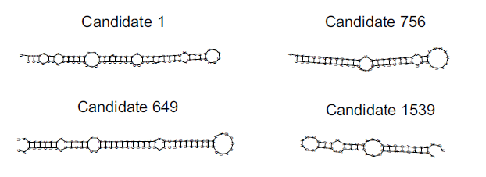
\includegraphics{p6g.pdf}
\end{center}

\item Una empresa de videojuegos para redes sociales está realizando un análisis de sus clientes para determinar cuáles son los patrones que distinguen a aquellos que más viralizan (difunden el juego entre otros) y monetizan (pagan por características especiales). Para realizar este estudio, desde la aplicación envían a un servidor de la empresa una amplia variedad de datos acerca de los usuarios y su comportamiento. En relación a las categorías de usuarios se envía la edad, sexo, país de origen, etc. En cuanto al comportamiento, el servidor recibe permanentemente datos sobre: instalación y desinstalación del juego, entradas y salidas, invitaciones enviadas, invitaciones aceptadas, menciones del juego en el muro del usuario, número de clics en diferentes regiones predefinidas, entradas a publicidad, dinero recibido por características especiales, etc. Con toda esta información se requiere encontrar perfiles característicos de usuarios y luego determinar cuáles son los patrones de comportamiento que definen a los usuarios que viralizan y monetizan más. Finalmente, a partir de estos patrones de comportamiento se pretende desarrollar un predictor de viralización y monetización que permita saber con suficiente anticipación qué usuarios
deben ser atendidos especialmente, por ejemplo mediante regalos o algún tipo de publicidad especialmente dirigida.

\item Se desea modelar una epidemia de cólera ocurrida en Buenos Aires en 1867. Se ha tratado de reconstruir la situación pero la clara no linealidad en la dinámica y la falta de un registro completo de las variables a hecho fracasar todos los intentos realizados a partir de los modelos matemáticos más tradicionales. Básicamente, se sabe que la epidemia se habría iniciado en Rosario y San Nicolás y aparentemente ingresó a Buenos Aires a través del barrio de La Boca. Se poseen algunos registros históricos incompletos acerca de la cantidad de pacientes con síntomas de cólera detectados día a día en estas tres ciudades y la cantidad de muertos en Buenos Aires, aproximadamente cada 15 días y durante 6 meses. Se solicita que diseñe una arquitectura neuronal para modelar este fenómeno y proponga todas las etapas para la preparación de los datos, entrenamiento y validación del modelo.

\item Proponga un modelo que aprenda la estructura de múltiples comunidades en una red social y que, en función de lo aprendido, pueda hacer sugerencias de asociación a los usuarios.

\item Se desea desarrollar un predictor de precipitaciones que utilice como entradas las series de precipitaciones y temperaturas medias diarias del último mes, por un lado, y la presión atmosférica y los índices de nubosidad correspondientes a los últimos 7 días. Proponga una método para realizar dicha predicción, especificando claramente todas las etapas de la solución propuesta y los métodos de entrenamiento y validación, si los hubiere.

\item Un grupo de productores agrícolas está estudiando la forma óptima de combatir las plagas en sus sembrados sin afectar significativamente el rendimiento. Para ello, han digitalizado la imagen de una gran cantidad de hojas con distintos tipos y grados de daño producido por varias especies de plagas. Para cada imagen se posee la recomendación del especialista en cuanto a la dosis y composición del insecticida a aplicar. Se solicita que proponga un método automático para obtener estos datos a partir solamente de la imagen digitalizada. Describa detalladamente todos los pasos a seguir, las arquitecturas y los métodos de entrenamiento y validación propuestos.

\item A partir de una base de datos que contiene todos los registros de compras de un gran supermercado, se desea poder encontrar automáticamente los principales perfiles de cliente y luego clasificar una determinada lista de compras según éstos perfiles. Además, dado un determinado perfil, se desea ofertar otros productos que estén relacionados a los comprados por los consumidores dentro del perfil. Proponga los modelos necesarios, con sus métodos de entrenamiento y aplicación, para: encontrar los perfiles automáticamente, clasificar las listas de compras y determinar productos relacionados para ofertar.

\item En una editorial se está realizando una reestructuración del depósito y para eso se requiere un sistema capaz de sugerir las categorías de libros a ser almacenados en una misma estantería o en estanterías cercanas. Se cuenta con el historial de ventas de los últimos 10 años, incluyendo datos como: título, autor, género, fecha de ingreso, cantidad de ejemplares vendidos por mes, precio, cantidad total de páginas, dimensiones, peso, etc.

\item En una gran base de datos de transacciones bancarias se desea encontrar patrones de comportamiento que sirvan de apoyo a la toma de decisiones relacionadas con diferentes inversiones que realizarán dos corporaciones internacionales. Proponga una metodología para extraer información de relevancia, la arquitectura neuronal a utilizar y el método de entrenamiento.

\item Se desea modelar una epidemia de cólera ocurrida en Buenos Aires en 1867. Se ha tratado de reconstruir la situación pero la clara no linealidad en la dinámica y la falta de un registro completo de las variables a hecho fracasar todos los intentos realizados a partir de los modelos matemáticos más tradicionales. Básicamente, se sabe que la epidemia se habría iniciado en Rosario y San Nicolás y aparentemente ingresó a Buenos Aires a través del barrio de La Boca. Se poseen algunos registros históricos incompletos acerca de la cantidad de pacientes con síntomas de cólera detectados día a día en estas tres ciudades y la cantidad de muertos en Buenos Aires, aproximadamente cada 15 días y durante 6 meses. Se solicita que diseñe una arquitectura neuronal para modelar este fenómeno y proponga todas las etapas para la preparación de los datos, entrenamiento y validación del modelo.

\item Considere un problema de reconocimiento óptico de caracteres (OCR) donde se requiere reconocer texto manuscrito en frases aisladas de entre 5 y 10 palabras. Proponga dos arquitecturas neuronales dinámicas para la solución de problema y detalle todos los pasos desde la preparación de los patrones de entrenamiento hasta las pruebas de validación.

\item Proponga un sistema de reconocimiento que pueda ser entrenado con datos de diferente naturaleza (sonidos, imágenes, texto, etc).
\end{enumerate}

\end{document}